% A 15-puzzle made from one illustration (not experimental data).
% Source tile numbers run left to right, top to bottom. Tile 16 is omitted.
% Starting with the vacancy at lower right, move it L, U, R, U, L, D.
% Each nonzero entry below uses its entire source tile without rotation.
\begin{tikzpicture}[x=1cm,y=1cm]
  \definecolor{puzzleRim}{HTML}{293644}
  \definecolor{puzzleTray}{HTML}{BAC6CB}
  \definecolor{puzzleSlot}{HTML}{82939E}
  \fill[rounded corners=1.5pt,fill=puzzleRim] (-.09,-.09) rectangle (4.186,4.186);
  \fill[rounded corners=.65pt,fill=puzzleTray] (-.025,-.025) rectangle (4.121,4.121);
  \foreach \piece [count=\location from 0] in
    {1,2,3,4,5,6,12,7,9,10,0,8,13,14,11,15}{
    \pgfmathsetmacro{\destX}{mod(\location,4)*1.032}
    \pgfmathsetmacro{\destY}{(3-floor(\location/4))*1.032}
    \begin{scope}[shift={(\destX,\destY)}]
      \ifnum\piece=0\relax
        % Unmarked recessed space into which an adjacent tile can slide.
        \fill[puzzleSlot] (0,0) rectangle (1,1);
        \fill[puzzleTray] (.026,0) rectangle (1,.974);
      \else
        \pgfmathtruncatemacro{\sourceX}{mod(\piece-1,4)}
        \pgfmathtruncatemacro{\sourceY}{3-floor((\piece-1)/4)}
        \begin{scope}
          \clip[rounded corners=.45pt] (0,0) rectangle (1,1);
          \node[anchor=south west,inner sep=0pt,outer sep=0pt]
            at (-\sourceX,-\sourceY)
            {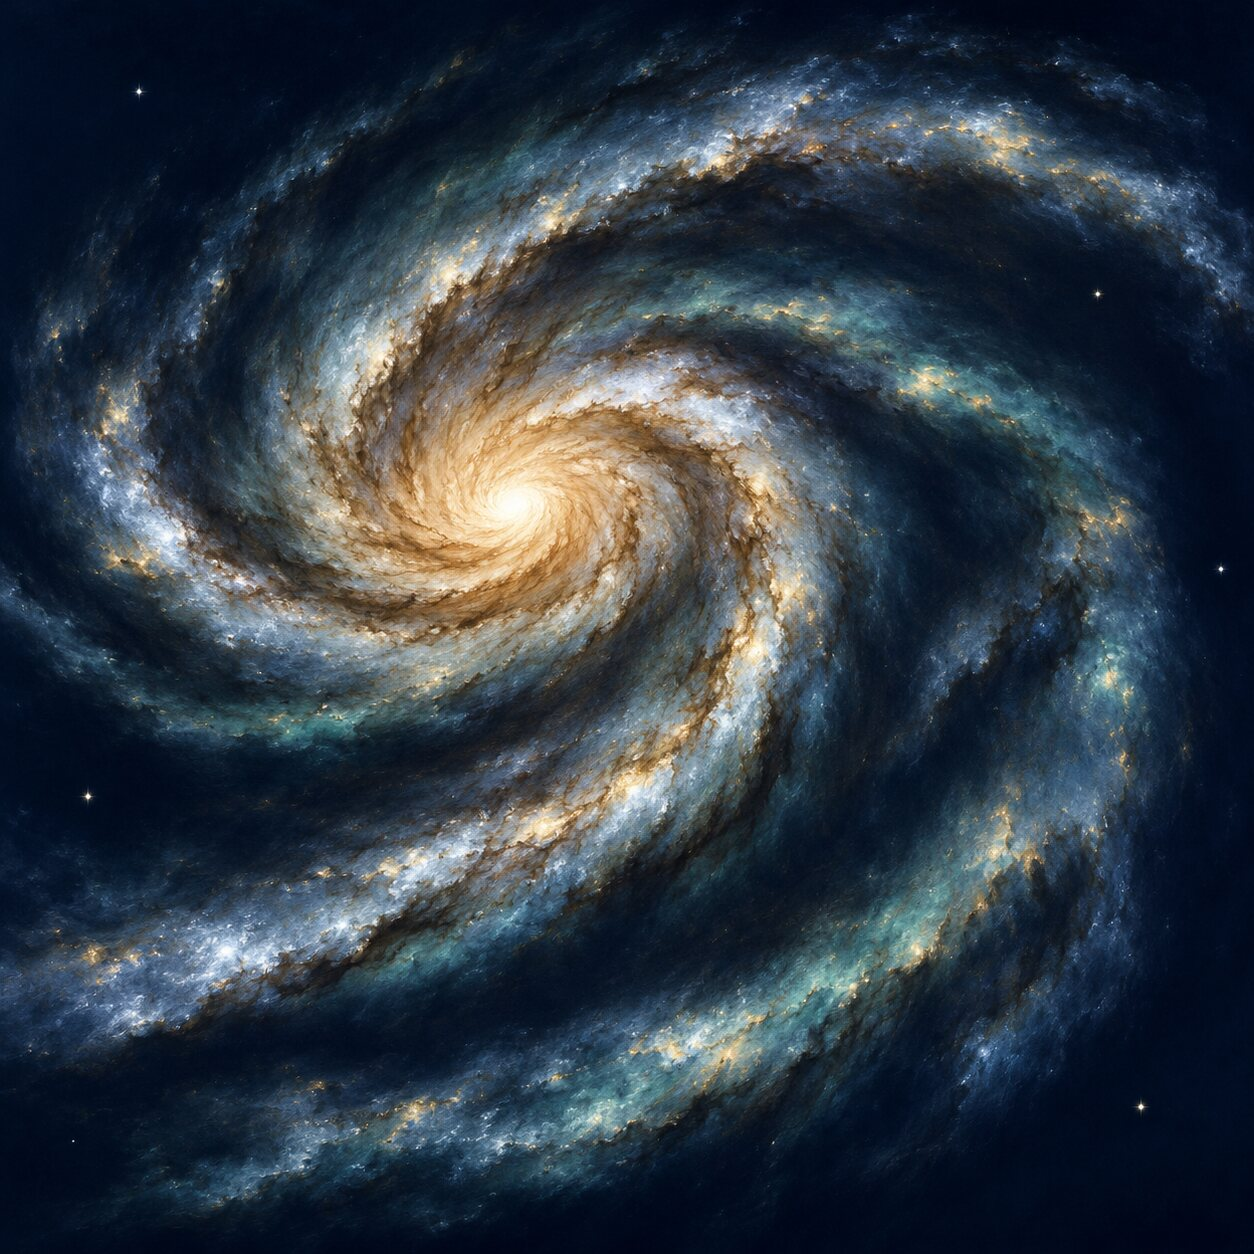
\includegraphics[width=4cm,height=4cm]{figures/galaxy-art.jpg}};
        \end{scope}
      \fi
    \end{scope}
  }
  \pgfresetboundingbox
  \path[use as bounding box] (-.09,-.09) rectangle (4.186,4.186);
\end{tikzpicture}%
